\documentclass[10pt]{book}
\author{Marco Perronet - Stefano Chiavazza}
\title{Process scheduling in the Linux Kernel}
%Stefano
% "Qualche differenza
%

%Marco
% 
% Linux Kernel: Monitoring the Scheduler by \verb|trace_sched*| Events

\usepackage[utf8]{inputenc}
\usepackage[english]{babel}
\usepackage{microtype}
\usepackage{fancyref} % for refs
\usepackage{graphicx} % for including pictures
\graphicspath{ {./images/} }
\usepackage{amsmath} % useful for math
\usepackage{pgfplots} % for plots
\usepackage{booktabs} % good for beautiful tables
% packages for code
\usepackage{verbatim}
\usepackage{fancyvrb}
\usepackage{minted}
\usepackage{hyperref}
% code style
\newminted[code]{c}{frame=single, 
framesep=2mm,
baselinestretch=1.2,
breaklines, 
breakafter=d,
linenos
}

\begin{document}
\maketitle
\tableofcontents
\textbf{Abstract}\\
This thesis is about scheduling and its implementation in the Linux kernel. Other related topics
will be covered, such as kernel architecture and event tracing, an important aspect of kernel debugging. %write here an excitiong oneliner about what we're gonna do in the thesis
The focus will be on explaining how the current scheduler in the kernel works, as well as documenting scheduling-related events.
The two are strictly related to each other. You cannot, of course, document these events without understanding how the scheduler works: this is 
why most of them will be mentioned and explained on the fly, while discussing other concepts.

Examples in the code will always be provided, each piece of theory will have its implementation counterpart shown and explained.
Most of the concepts are very easy to visualize once the code is split into its most significant parts
and then dissected line by line, however, this is not an internals manual for development. 
This thesis should be considered a guide. It's meant for people who are curious about the inner workings of the kernel
but have never looked too much into it, its goal is to give interesting insights about the architecture of operating systems.
The only prerequisite is to have some experience with C and know the very basics of GNU/Linux and operating systems.

All references to the source code are from kernel version 4.20.13, the latest stable version at the time of writing. When discussing architecture dependent code it will be assumed that the architecture is x86. In the code, every multiline comment (\verb|/*...*/|) is written by the kernel developers, my comments will always be inline (\verb|//|).

%Explain how the thesis is structured
In the first part I will give a brief overview of the kernel and then explain some basic scheduling concepts.\\
\dots (will write this at the end)
\dots\\
Here is a useful tool to quickly look up mentioned kernel functions for yourself \texttt{elixir.bootlin.com/linux/v4.20.13/source}. Another alternative is to download the whole source code from \texttt{kernel.org}, which is needed if you want to compile and load it. 

\chapter{Basics of Linux kernel}
\label{ch:introduction}

\section{Operating Systems}
\label{sec:os}
The operating system (OS) comprises the software intended to manage the hardware resources and the \textit{application software}, which performs specific, high level tasks. The application software, which is the larger part of the OS, is made of utility programs and any other software with which you interact directly. These programs are not part of the core OS, but they are necessary to do anything useful. The operating system acts as an intermediary between the user and the machine by abstracting away the hardware, which makes interaction easier: this is why almost every computer runs an operating system.

It can be argued that the OS is not strictly necessary because it's possible to execute a program without loading an OS: this is referred as \textit{bare metal programming} and it's common in embedded systems. Because there is no operating system (which means no filesystem, memory management or any useful application), programs cannot be written on the system itself. Instead, the program is written on another machine with an operating system, then compiled with a cross-compiler, which will compile for an architecture different than the one it is running on. Finally, the compiled binaries are loaded at boot time on the target embedded system. This is the opposite of what we are used to: being able to reprogram the machine as it is running, by writing and compiling our program with \textit{application software} designed to edit text and compile code. Thus, an operating system greatly simplifies interaction with the machine by offering a platform for the user and, at a higher level, by making general-purpose computing possible. There are also OSes for embedded systems called \textit{real-time systems}, but we will focus only on general-purpose OSes. 

Windows, MacOS, iOS, Android... Most of us are familiar with these operating systems. Besides the platform on which they run, they are all general-purpose and their goal is the same; what really changes is the architecture and philosophy in their design. At a macroscopic level they differ in kernel design approach (monolithic kernel vs hybrid kernel), but we need to wait until the next section to see what this means. At a microscopic level, there is literally not much to see because the code of most OSes is closed, so it's impossible to see the implementation differences with Linux. This leads us to one of the peculiarities of Linux: it's completely open source and community developed. Besides---not really interesting---ethical matters, this means that it's possible to study the code and get a full understanding of operating systems. In fact, before Linux, there was no way to see how operating systems work in practice. The only option was to study them from textbooks in order to implement your own kernel, which is exactly what Linus Torvalds did.

We said earlier that a key component of an OS is ``the software intended to manage the hardware resources'': this is what we refer as the \textit{kernel}. Dennis Ritchie, the creator of Unix and C, also called it the ``Operating system proper''\cite{ritchie}, which most likely means ``The component that is the actual operating system''. One one hand it's true, because the low level tasks performed by the kernel are essential (and also because it's the most difficult component to develop), but on the other, without application software the kernel is useless. You can load a kernel at boot, then it initializes and starts running, and then there is nothing but a black screen because there is no other program to start. So no, it's not an operating system by itself, but what Dennis meant is that when you think about the core architecture of an OS, you think about the kernel. An engine is indeed useless without the rest of the car, but does that make the other components as important as the engine, where all the complexity resides? Despite the application software being the largest part of the OS; it is within the kernel that the hardest engineering challenges are found, which makes it the most interesting---and difficult---part to understand and analyze.

\section{A general overview} 
\label{sec:general}
The kernel's job is to manage hardware resources, which means handling all interactions with the CPU, memory and I/O devices. More specifically, the kernel needs to respond to I/O requests, manage memory allocation and decide how to share CPU time. To achieve this, it has access to all resources in the system, which is needed to make the most out of hardware: its performance is what makes the difference between a fast or a slow operating system. This critical role requires a protection mechanism to ensure the stability of the whole system: this is achieved by separating kernel code and user application code. In practice, depending on your configuration at compile time, what happens is: 
\begin{enumerate}
    \item The kernel binary image will be loaded in RAM in a low or high memory area.
    \item A predefined slice of RAM next to that memory zone will be reserved for the kernel. 
    \item The remaining part of the memory will be accessible to the user.
\end{enumerate}
These two parts of RAM are called kernel space and user space. The former is a reserved area dedicated to critical system tasks and it's protected from user access, the latter is the area where system utilities and user programs run. This memory partitioning makes sure that kernel and user data do not interfere with each other, and it is also a security measure because it prevents a malfunctioning or malicious user program from crashing the entire system.

\subsection{System calls} By extension of this design, interaction with user space is regulated with a privilege system: each process can run either in user mode or kernel mode. Processes running in user mode can access privileged kernel functionalities through special gates in a predefined and controlled manner: these gates are implemented as functions called \textit{system calls}, which serve as an API between user and kernel space. When a user process performs a system call it will temporarily execute in kernel mode, perform tasks that require a high privilege, and then switch back to low privilege. This mechanism is implemented at a hardware level: in the x86 architecture 2 bits in the code selector (\verb|cs|) register indicate the current privilege level (CPL) of the program that is running on the CPU. This value is 0 or 3, respectively, for kernel and user mode and each system call will change this value temporarily. 

\begin{figure}[ht]
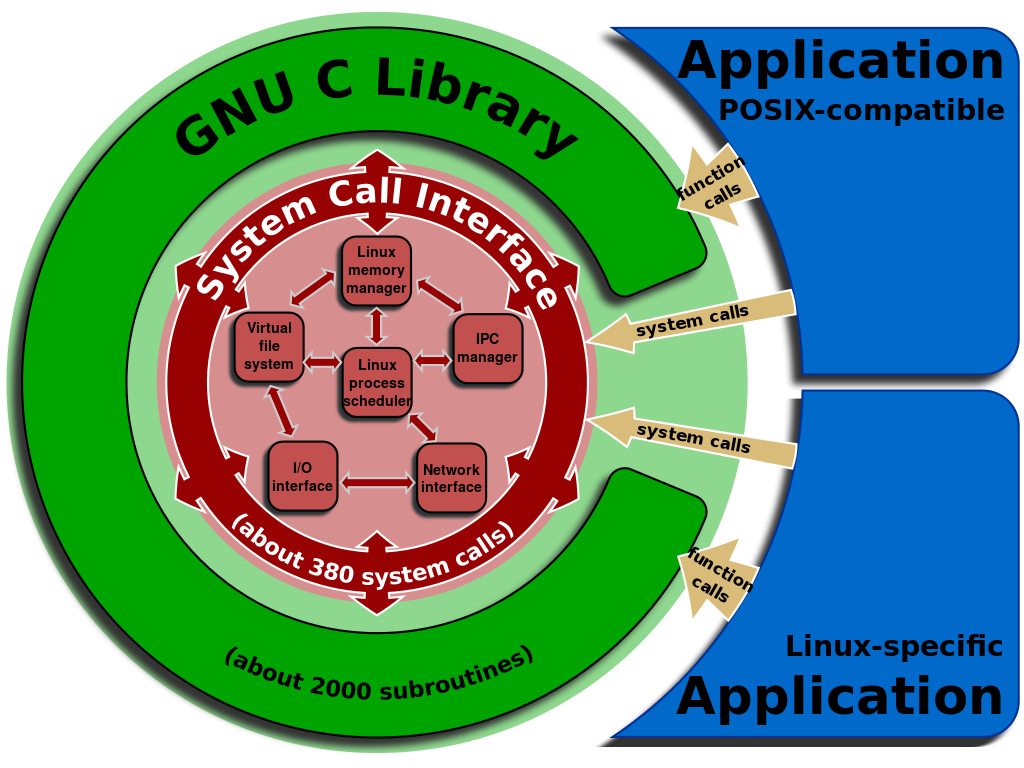
\includegraphics[width=\textwidth]{images/userspace_kernelspace.png}
\caption{Kernel space (in red) and user space (in green and blue)}
\label{img:userspace_kernelspace}
\end{figure}

Any useful operation in the system requires privileged services from the kernel. In fact, an extremely simple shell command such as \verb|echo| performs dozens of system calls. It's easy to see this by executing \verb|strace -wc [command]|, which will show each system call performed by \verb|[command]| during its execution. System calls can be called in user space applications directly, through assembly, or indirectly, by calling wrapper functions from the C standard library (\verb|glibc|), as shown in Figure\ref{img:userspace_kernelspace}. 
\begin{code}
// Two different ways of calling open/close through glibc wrapper functions 
// SYS_open and SYS_close correspond o the syscall numbers
int fd = syscall(SYS_open, "example.txt", O_WRONLY);
syscall(SYS_close, fd);
fd = open("example.txt", O_WRONLY);
close(fd);
\end{code}
Calling through assembly means filling the right CPU register with the syscall arguments and then using a special instruction. On x86 it's \verb|int $0x80|, though modern processors sometimes use a different one. This is what will happen upon its execution:
\begin{enumerate}
    \item Interrupt number 128 (\verb|0x80| in decimal) gets triggered. In Linux it corresponds to a system call interrupt. 
    \item The process execution is suspended and the control passes to the kernel (kernel mode), which will look up the entry 128 in the \textit{interrupt vector table}. This table simply associates interrupt numbers with their handler: a function that gets executed when the interrupt happens.
    \item The corresponding handler is executed: this function copies the syscall number and arguments from the registers onto the kernel stack. It will then look up in the \textit{system call dispatch table} the handler corresponding to the syscall number and call it with the correct arguments like any normal C function, because the arguments are now located on the kernel stack.
    \item The system call is finally executed and the return value is stored in a general purpose data register.
\end{enumerate}
Registers are used to pass the parameters because this way it's easier to get them from user to kernel space. It's intuitive that calling system calls this way is very architecture dependent since you're working on registers. This is why \verb|glibc| wrappers are always used: they internally execute the assembly code that we just discussed and do it differently for each architecture (you can write assembly into C source code, more on this later). Calling wrappers is also very safe since you can't accidentally fill the wrong registers or miss the right number of arguments and, moreover, most syscalls have a wrapper so there's no reason to write assembly for them. It's important to note that the kernel can protect itself against invalid syscall arguments in registers, which is crucial since, as we saw, you can easily call syscalls from user space directly by writing assembly.

\subsection{A different kind of software} The separation between kernel/user space and the fact that we are working at such low level makes the kernel a very peculiar piece of software. One of its properties is that there is no error checking, this is because the kernel trusts itself: all kernel functions are assumed to be error-free, so the kernel does not need to insert any protection against programming errors\cite{cesati}. What the kernel does instead is to use assertions to check hardware and software consistency; if they fail then the system goes into \textit{kernel panic} and halts. We will see later in the code some examples where the \verb|panic()| routine is called. A good reason for this choice is that since the kernel controls the system itself it's very hard to correct errors and, even then, error recovery code would take a huge part of the code. Another way of thinking about this is that there is no meta-kernel that handles kernel errors. Of course programming or hardware errors can (and will) still occur: when this happens the offending process is killed and a memory dump called ``\textit{oops}'' is created. A typical example of this is when the kernel dereferences a NULL pointer: in user space this would cause a \textit{segmentation fault}, while in the kernel it will generate an oops or in the worst case go directly into panic. After this kind of event, the kernel can no longer be trusted and the best thing to do would be to reboot, because the kernel is in a semi-usable state and it could potentially corrupt memory. Furthermore, a panic in this state is more likely to happen. %oops count after the first one?

% Ricordare di mettere parentesi quando si citano funzioni
Another peculiarity of the kernel is that it uses its own implementation of the functions in the standard C library. For example \verb|printf()| and \verb|malloc()| are implemented as \verb|printk()| and \verb|kmalloc()|. There are different reasons for this choice, one of those is that the C standard library is too big and inefficient for the kernel. Another reason is that implementing your own functions gives more freedom because they can be customized for their purpose in the kernel. Memory allocation in user or kernel space is very different, so the \verb|kmalloc()| implementation is very specific. For instance, kernel data structures need a contiguous physical memory segment to be allocated, while regular user space allocation doesn't have this restriction. Furthermore, \verb|printk()| writes its output into the kernel log buffer (that you can read by using the \verb|dmesg| command in user space); this is very different from \verb|printf()| that writes on standard output.

\subsection{A monolithic design}
%TODO, be brief, this is not so important but it's interesting

\subsection{User and kernel stacks} Before we begin, one last thing is important to understand. We already said that memory management in kernel/user space is different: the same is true about execution. Every process in the system has two stacks, located respectively in user and kernel space, and it will use one of the two while executing in the respective privilege mode. x86 CPUs automatically switch stack pointers when privilege mode switches occur, which usually happens for syscalls. The user space stack can potentially be very big, with a very high limit (8mb on my machine, but it can be increased), and even though it's initially small it can allocate more physical memory as it needs it. This mechanism is called ``on-demand paging'', we will discuss this topic and virtual memory in section \ref{sec:core}. The kernel stack, unlike the user stack, does not have the luxury to expand itself and has a fixed size of two pages. 32-bit and 64-bit systems have 4kb and 8kb sized pages, respectively, so the stack size is 8kb or 16kb. These two pages must be allocated contiguously, which can cause memory fragmentation for long system uptimes as stacks get deallocated. In other words, it becomes increasingly hard to find two physically contiguous unallocated pages as the OS runs for a long time. This is why in the past efforts have been made to reduce the stack size to one page, which would eliminate fragmentation, but after many stack overflows the standard settled on two pages. 

This leads us to an interesting example of the kernel trusting itself: it makes the big assumption that the stack will never overflow, \textbf{there is no protection against it}. So what happens if it overflows? First, it will corrupt the \verb|thread_info| data structure, which is the first thing that the stack encounters along its path (Figure \ref{img:stack}). This will make the process inexistent for the kernel and cause a memory leak (we will see why). Next, the stack can overflow outside of the address space and silently corrupt whatever kernel data is stored; the best case scenario here would be a kernel panic to prevent any further memory corruption. Another natural question might be ``why are kernel stacks so small?'' and the answer is simple: first, to use a small amount of kernel memory, and secondly, because of fragmentation. The bigger is your data structure in contiguous physical memory, the more it is hard to allocate. It is expected that any process stays in kernel mode for a small amount of time, so it should use a very small portion of the stack. A consequence of small stacks is that very few recursive functions are used to avoid long call chains and minimize stack usage; the same is true for big static allocations on the stack. %check this

\begin{figure}[ht]
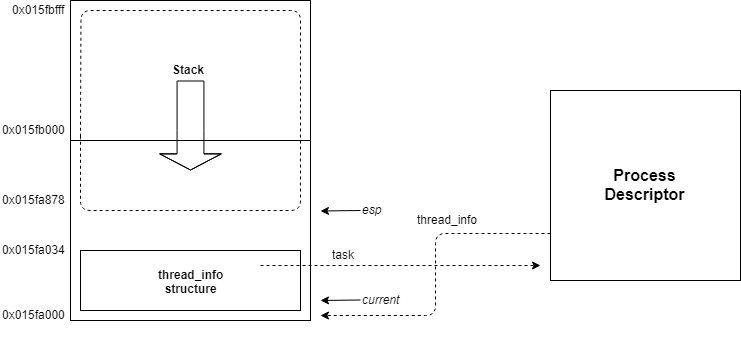
\includegraphics[width=\textwidth]{images/stack.png}
\caption{The kernel stack inside its small address space of two pages, it grows downward towards low memory.}
\label{img:stack}
\end{figure}

It's important to note that there are special processes called \textit{kernel threads} that do not follow this pattern of kernel/user stack. Kernel threads perform a specific system task, they are created by the kernel and they live exclusively in kernel space, never switching to user mode. Their address space is the whole kernel space and they can use it however they want. Besides this, they are normal and fully schedulable tasks just like the others. An example of a kernel thread is \verb|ksoftirqd|: there is always one for each CPU and their job is to dispatch interrupt requests. As a side note, the name stands for ``Kernel Software Interrupt ReQuest Daemon'', many kernel threads follow a similar naming convention. %mention per-CPU kernel stacks for handlers?
%Interrupt stacks - To rectify this problem, the kernel developers implemented a new feature: interrupt stacks. Interrupt stacks provide a single per-processor stack used for interrupt handlers. With this option, interrupt handlers no longer share the kernel stack of the interrupted process. Instead, they use their own stacks. This consumes only a single page per processor.
\section{Process management}
The kernel is divided into subsystems that interact with each other. Figure \ref{img:kernelmap} is a zoom into the kernel mechanisms inside the red part of Figure \ref{img:userspace_kernelspace}. The image represents the part of the kernel that will be covered, for the most part we will swing between the scheduling and memory mapping subsystems. The names in the picture are structs, functions or source code files; we will get familiar with most of these as we go on.

\begin{figure}[ht]
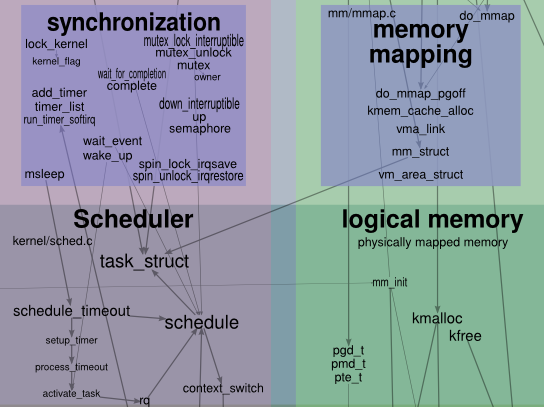
\includegraphics[width=\textwidth]{images/kernelmap.png}
\caption{A portion of the kernel subsystems map}
\label{img:kernelmap}
\end{figure}

\subsection{Processes and threads} A process is an instance of a running program. Each process has resources associated with it, such as an address space, open files, global variables and code. Each process must have its own address space that only he can access: when a process tries to access a memory location that does not belong to it, a segmentation fault interrupt is generated. A thread is defined as a single flow of execution, it has associated a stack of execution and the set of CPU registers that it uses, most notably the stack pointer and program counter. Each process can have multiple threads, in which case it's a \textit{multi-threaded process}; threads belonging to a process will share resources between each other. The execution aspect of a process is always represented by threads, which means that a process cannot exist without at least one thread associated.

The kernel doesn't distinguish between processes and threads, so they are treated as the same entity. Because of this a problem in terminology arises, so let's see how processes and threads are identified in practice.

Each process has its own PID (process id) and groups of processes are identified by the TGID (thread group id). If a process has only a single thread then its PID is equal to its TGID. If a process is multi-threaded then each \textit{thread} has a different PID, but they will all have the same TGID. Furthermore, there will be a thread in this group called \textit{thread group leader} that will have its PID equal to the TGID, so the TGID field in each thread is just the PID of their leader. Just to add some more confusion, when you call \verb|getpid()| you are actually getting the TGID (the group leader PID, identifying the whole process), and when you call \verb|gettid()| you are getting the PID (which identifies a single thread, not a group). So the PID is actually more like a thread identifier, that is also used as a process identifier when you have many threads associated to a process. This weird way of using ids was implemented to comply with POSIX standards, which require that each thread of a multi-threaded process must have the same id: this is why \verb|getpid()| returns the TGID.

You can already see how ``process'' and ``thread'' are being used interchangeably. As anticipated, this terminology can be confusing so let's clarify. A thread can be thought as a special kind of process, the real difference between the two is that threads share the same address space. Saying that some threads are associated to a process just means that they are sharing an address space: this is what enables concurrent programming and why synchronization methods are needed. As we will see shortly, using threads in a program instead of spawning new processes results in much better performance, which is why threads are sometimes called \textit{lightweight processes} or LWP. %wait, what if the thread stacks in the same address space overlap?
\begin{code}
//spawns a new thread
clone(CLONE_VM | CLONE_FS | CLONE_FILES | CLONE_SIGHAND, 0); 
//spawns a new process, this is the same as using fork()
clone(SIGCHLD, 0); 
\end{code}
The system call \verb|clone()| spawns a new child process. It's very similar to \verb|fork()| but it's more versatile because flags can be used to decide how many resources are shared with the new process. \verb|CLONE_VM| (where vm stands for virtual memory) makes the child process run in the same address space as the father, while the other flags clone filesystem information (such as working directory), open files and signal handlers. In line 4, \verb|SIGCHLD| simply means that the child process should send the \verb|SIGCHLD| signal to its father when it terminates. Ultimately, the reason why in Linux threads and processes are treated as the same entity, is that processes are just threads that share nothing. In fact, the word \textit{task} is always used inside the kernel instead of process/thread and we will do the same, especially when discussing implementation.

Each task is represented in the kernel with the struct \verb|task_struct|, this is a fairly big structure that can be almost 2kb in size, depending on configuration at compile time. \verb|task_struct| is what is often referred as the \textit{process descriptor} or PCB (\textit{process control block}): every information about a task is stored in here. 
\begin{code}
struct task_struct {
	/* -1 unrunnable, 0 runnable, >0 stopped: */
	volatile long			state;
	void				*stack;
	/* Current CPU: */
	unsigned int			cpu;
	// A boolean, "on_runqueue"
	int				on_rq; 
	int				prio;
	int				static_prio;
	int				normal_prio;
        int				exit_state;
	int				exit_code;
	int				exit_signal;
	/* The signal sent when the parent dies: */
	int				pdeath_signal;
	pid_t				pid;
	pid_t				tgid;
        /* Real parent process: */
        // The original parent that forked this task
	struct task_struct __rcu	*real_parent;
	/* Recipient of SIGCHLD, wait4() reports: */
	// The current parent, maybe the original one exited
	struct task_struct __rcu	*parent;
	// Executable name, usually the command that spawned this task
	char				comm[TASK_COMM_LEN]; 
        /* Filesystem information: */
	struct fs_struct		   *fs;
	/* Open file information: */
	struct files_struct		*files;
	/*
	 * Children/sibling form the list of natural children:
	 */
	struct list_head		children;
	struct list_head		sibling;
	struct task_struct	   *group_leader;
	/* PID/PID hash table linkage. */
	struct pid			*thread_pid;
	struct hlist_node	   pid_links[PIDTYPE_MAX];
	struct list_head		thread_group;
	struct list_head		thread_node;
};
\end{code}
\verb|include/linux/sched.h|

These are some of the most basic fields the struct, most of them are self explanatory.

The \verb|volatile| keyword basically tells the compiler to not over optimize by caching the value of this variable, it indicates that the value may change even if the variable does not appear to have been modified. This means that every time the variable is accessed it needs to be read from the main memory, and it will never be stored in a CPU cache. The opposite of \verb|volatile| is the compiler hint \verb|register|. The fact that the task state is volatile makes sense because it could be unpredictably modified by interrupts: it could be possible that an old value of the variable is read from the cache instead of the actual value.

Let's now focus on the pid fields to show how Linux uses pids to find any information and resources of a task. Given a pid, searching linearly through the pids to find the task we are looking for would be very inefficient. Instead, a hash table known as \textit{pid hash table} is used. The identifiers in this table are simply the result of hashing a given pid, you can see in figure \ref{img:pidhash1} that conflicting entries are simply stored in a list associated with the same id. Because it's a hash table, the kernel can quickly look up the pid and find in $O(1)$ time the corresponding process descriptor. This is exactly what happens when you use shell commands such as \verb|kill [PID]|.

\begin{figure}[ht]
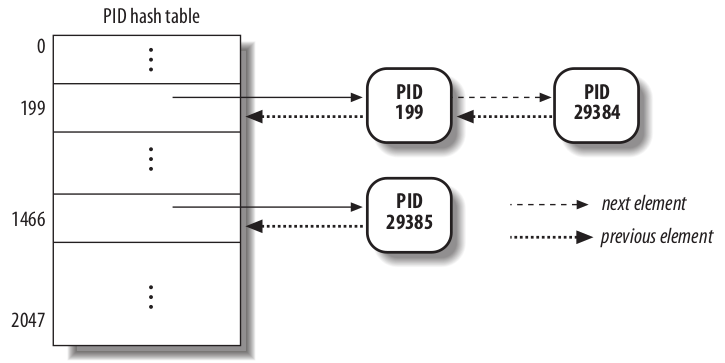
\includegraphics[width=\textwidth]{images/pidhash1.png}
\caption{Pid hash table, pids 199 and 29384 are both hashed to 199}
\label{img:pidhash1}
\end{figure}

\begin{code}
enum pid_type {
	PIDTYPE_PID,  //process PID
	PIDTYPE_TGID, //thread group leader PID
	PIDTYPE_PGID, //process group leader PID
	PIDTYPE_SID,  //session leader process PID
	PIDTYPE_MAX
};
\end{code}
\verb|include/linux/pid.h|

There are actually four tables, one for each PID type. Each of these tables is an array of \verb|hlist_head|, the head of the chain list, which points to a list of \verb|hlist_node| (see figure \ref{img:pidhash2}). These are the structures used for non-circular lists. These lists are populated by \verb|struct pid|, and a pointer to this struct is stored inside each process descriptor in the \verb|thread_pid| field. Figure \ref{img:pidhash2} shows and example for the TGID class that we discussed earlier. Pids in the chain list are colliding and are different processes, pids in the \verb|pid_list| are threads in the same group, where the leftmost thread in the image is the group leader. Don't be fooled by the name ``\verb|list_head|'' inside the pid structure, it's actually a list \textbf{node} of a circular list, and since it's circular there's really no head structure that points to the first element. %CHECK THIS

\begin{code}
struct pid {
        atomic_t count; // number of references to this PID
	int nr; // PID number
	struct hlist_node pid_chain; // Link to next and previous conflicting entries
	struct list_head pid_list;  // per-PID list
};
\end{code}
\verb|include/linux/pid.h|

\begin{figure}[ht]
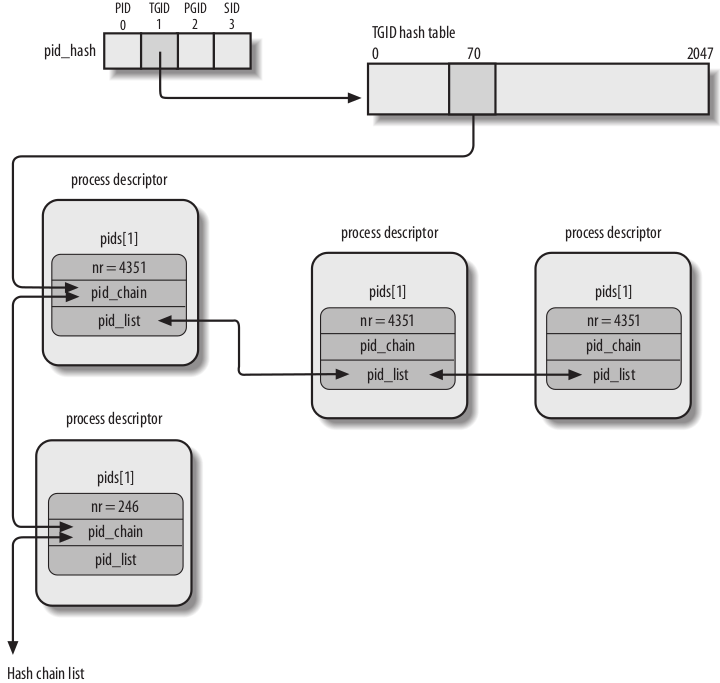
\includegraphics[width=\textwidth]{images/pidhash2.png}
\caption{Hash table for the TGID pid type}
\label{img:pidhash2}
\end{figure}

The implementation of \verb|struct pid| is actually a little different than what I presented, with other nested structures and a different linkage to the hash table. The way pids are organized is conceptually the same so I presented it like this for semplicity's sake. In this section we covered a small piece of the process descriptor, we will thoroughly examine the other fields in section \ref{chap:implementation}.

%the thread_pid field is a pointer so the struct pid is not actually embedded in the process descriptor, yikes! maybe take a look at this later
%don't use struct pid as an example here for now...

%maybe move this section for later?
\subsection{List implementation} In a classic circular list you would have a struct with your data and then pointer to next and prev nodes. This implementation is naive and would lead to have a different structure for each data type, or using a void pointer to your data for no reason. Let's see how lists are used in the kernel.

\begin{figure}[ht]
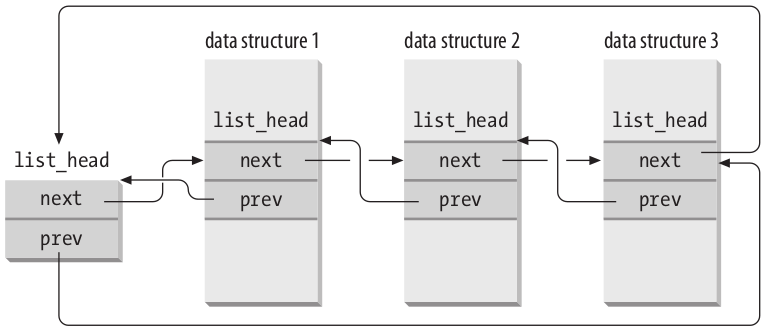
\includegraphics[width=\textwidth]{images/list.png}
\caption{A generic doubly linked circular list}
\label{img:list}
\end{figure}

\begin{code}
struct list_head {
	struct list_head *next, *prev;
};
\end{code}
The data is not contained in the list itself, but in another structure that contains the list node (Figure \ref{img:list}). For example, Linux keep a big circular list of every \verb|task_struct| in the system: this is done by embedding ``\verb|struct list_head tasks;|'' into \verb|task_struct|. Notice how this is not a pointer to a node: the node is embedded directly into the structure. So how can we get the data we want in the structure without a pointer in the node? The answer is the \verb|container_of()| macro. This macro works with anything, but let's assume that we have a list embedded in the container structure.
\begin{code}
#define container_of(ptr, type, member) ({ \
	void *__mptr = (void *)(ptr); \
	((type *)(__mptr - offsetof(type, member))); })
// An alias that's used everywhere
#define list_entry(ptr, type, member) \
        container_of(ptr, type, member)
\end{code}
\verb|include/linux/kernel.h|
ptr is the pointer to the list node, type is the container struct, member is the field name of the list node in the container struct. We first cast ptr to a void pointer, then we subtract the offset from the beginning of the container struct of the field we want to get. When we allocate a struct, its field are allocated contiguously in virtual memory in the order that we declared them: this means that by moving the pointer backwards from a field by the right amount, we can end up at the beginning of the container structure. This is how we can get the offset of the a specified field in any struct. 
\begin{code}
#define offsetof(TYPE, MEMBER) ((size_t)&((TYPE *)0)->MEMBER)
\end{code}
\verb|include/linux/stddef.h|
TYPE is the struct we are considering, MEMBER is the name of the field, what it does is:
\begin{enumerate}
    \item Take the address 0, the first in the address space of the process
    \item Cast it to a TYPE pointer 
    \item Dereference the pointer and take the MEMBER field
    \item Take the address of the field and cast it to a size, now it's no longer an address
\end{enumerate}
Essentially, we are pretending that there is the container structure allocated just at the beginning of the address space. This is arguably a bit of a hack, but it's perfectly safe since we are just playing with pointers and never touching actual memory. Indeed, it would be very dangerous to dereference and modify data from a random pointer in memory. This approach has many advantages, such as being able to have multiple lists associated with the same data. \verb|task_struct|, for instance, contains also the \verb|children| and \verb|sibling| lists among many others. This implementation is also very easy to use and it's oblivious about types.

%Mention cooperative multitasking?
\subsection{Scheduling} A system with a single CPU can handle only one process at a time and this is why it's needed to schedule processes. Process scheduling consists in choosing which processes should run in what order, essentially deciding how CPU time is shared between processes. To achieve this, there are many scheduling algorithms such as FCFS (\textit{first come first served}), RR (\textit{round robin}), EDF(\textit{earliest deadline first}) and SJF (\textit{shortest job first}). Most of the scheduling policies are \textit{preemptive}, which means that at any time the scheduler can arbitrarily decide to interrupt the currently running task and assign the CPU to another process. The use of preemption implies that processes have assigned \textit{timeslices}: they are periods of time in which the process is allowed to run and after which it will be preempted. FCFS, which is the most basic scheduling algorithm, doesn't have preemption nor timeslices: every process will run as much as it wants before voluntarily giving up the CPU to the next task in the queue. Round robin is similar to FCFS because it has a FIFO runqueue; the difference is that it uses a constant timeslice, called \textit{quantum}, assigned to each process: when the quantum expires the process gets preempted and the next task is scheduled.

In an UP (\textit{uniprocessor}) system it's impossible to achieve true parallelism. The only way to do it is to have multiple processors that share a common bus and the central memory: this is known as SMP (\textit{symmetric multiprocessing}). A single processor can also have multiple cores, but each one is treated as a separate processor, so the SMP architecture applies to cores as well. Even on SMP systems, which represent most systems today, you're always going to have more processes than cores, so scheduling is necessary for each processor/core. There are also new problems that arise in SMP, such as \textit{load balancing}: the problem of balancing processes between CPUs so that no CPU goes idle or has an unfair amount of workload. These kind of related problems must also be taken into account by the scheduler.

Every job carried out by the scheduler will eventually lead to a process switch on a given CPU. The kernel has a mechanism to suspend the execution of a process, save its status, and resume another process: this procedure goes by the name of \textit{context switch}. Each process has an \textit{execution context}, which includes everything needed for a task to execute, from its stack to the code. While every process can have its own process descriptor, the registers on the CPU must be shared between every process in the system. Every value in any register that a process is using is a subset of the execution context and it's called the \textit{hardware context}. At every context switch the hardware context must be saved and restored, respectively, for the old and the new process. The content of the registers are saved in part in the process descriptor of the preempted process, and in part on its kernel stack.

The routine that performs a context switch is called---not surprisingly---\verb|context_switch()|, and it's called only in one well-defined point in the kernel: inside the \verb|schedule()| routine, which triggers the scheduler and chooses the next task to schedule. \verb|context_switch()| (as we will see the code later) basically switches the address spaces of the two processes and then calls \verb|__switch_to()|. This last function operates on registers and kernel stacks, so it's one of the most architecture dependent in the whole kernel. This is why, like many other similar routines, there is one version for each architecture supported by Linux in the \verb|arch| folder. I don't want to go into assembly land and stick to C so we'll give a high level view of the procedure on x86, though it's important to know some of the registers in the x86 architecture. %why?

%TODO This part is too much, should I make it smaller or delete it? (probably delete it)
\textbf{Questa parte sui registri è inutile e pesante. Molto probabilmente la cancellerò}
There are 6 \textit{segmentation registers} that hold \textit{segment selector}, basically the starting address of memory segments in the process address space.
\begin{itemize}
    \item \verb|cs| \textit{Code segment}, this points to the segment containing instructions of the loaded program, also known as the \verb|.text| section. We mentioned in section \ref{sec:general} that this register also holds 2 bits that describe the current privilege level of the CPU.
    \item \verb|ss| \textit{Stack segment}, points to the the segment containing the stack of execution.
    \item \verb|ds| \textit{Data segment}, points to the the segment containing global variables and constants, also known as the \verb|.data| section.
\end{itemize}
The other 3, \verb|es|, \verb|fs| and \verb|gs| are general purpose are don't hold a specific address. There are also general purpose data registers that hold data used in operations (\verb|ax|, \verb|bx|, \verb|cx|, \verb|dx|) and pointer registers, that hold offsets:
\begin{itemize}
    \item \verb|ip| \textit{Instruction pointer}, offset to the next instruction. If added to \verb|cs| will be the address of the next instruction to fetch (\verb|cs:ip|).
    \item \verb|sp| \textit{Stack pointer}, offset to the top of stack. If added to \verb|ss| will be the address of the top of stack (\verb|ss:sp|).
    \item \verb|bp| \textit{Base pointer}, offset to subroutine parameters on the stack (\verb|ss:bp|).
\end{itemize}
Let's now see which part of the process descriptor is involved in context switching.
\begin{code}
struct task_struct {
    // ...
    /* CPU-specific state of this task: */
    struct thread_struct    thread;
};
\end{code}
\begin{code}
struct thread_struct {
#ifdef CONFIG_X86_32
    unsigned long	sp0;
#endif
    unsigned long	sp;
#ifdef CONFIG_X86_32
    unsigned long	sysenter_cs;
#else
    unsigned short	es;
    unsigned short	ds;
    unsigned short	fsindex;
    unsigned short        gsindex;
#endif
    // ...
    /* Floating point and extended processor state */
    struct fpu      fpu;
};
\end{code}
This struct is obviously very architecture dependent, its purpose is to save the hardware context before the context switch. You can see that even if it's specific to x86 it can still change depending on 32 or 64-bitness. You can also notice that only a small part of the hardware context gets saved in the process descriptor: the kernel stack pointer, general purpose segmentation registers, data segment and the floating point registers. In older versions of the kernel most of the registers were stored here.
Let's see in detail what happens when the kernel switches from process A to process B. There are actually two different mechanisms in this procedure: the entry/exit mechanism (user/kernel stack switch) and the context switch.
\begin{enumerate}
    \item Process A enters kernel mode, so it will switch from its user stack to its kernel stack, in other words: it saves its \textbf{user} hardware context in the kernel stack. It does so by pushing its \textbf{user mode} stack (\verb|ss:sp|), instruction pointer (\verb|cs:ip|) and data registers onto the kernel stack, then all CPU registers are switched to use the kernel stack.
    \item When in kernel context, process A invokes \verb|schedule()| which will eventually do \verb|context_switch()|.
    \item Process A saves its hardware context: 
    \begin{enumerate}
        \item It pushes most of its register values onto the kernel stack by a series of \verb|mov| assembly operations.
        \item It saves the value of the stack pointer (which is pointing to the \textbf{kernel} stack) into its \verb|task_struct->thread.sp|.
        \item Other registers such as the floating point registers are saved in the \verb|thread| field of \verb|task_struct|.
    \end{enumerate}
    \item Process A loads a previously saved stack pointer from process B's\\ \verb|task_struct->thread.sp|, also loads the other saved registers
    \item Address spaces are switched.
    \item Using the loaded stack pointer, process B moves its previously saved registers from its kernel stack into the registers. This is done by a series of \verb|pop [register]| assembly operations. Process B's state is now completely restored.
    \item process B exits kernel mode and restores its \textbf{user} context. This is accomplished by loading previously saved registers from the kernel stack: its \textbf{user mode} stack (\verb|ss:sp|), instruction pointer (\verb|cs:ip|) and data registers. Process B is now in user context.
\end{enumerate} %checka tutto ciò usando cesati TODO

To understand scheduling mechanisms in the next sections it's important to highlight something in step 2, when the scheduler gets called by a process running in kernel mode. It may be intuitive to think of the scheduler as some kernel thread that is permanently running in kernel mode, but that is not the case. \textbf{The scheduler does not run as a separate thread, it always runs in the context of the current thread.} This means that any process in the system that goes from/to kernel mode can potentially execute the scheduler himself, using its own kernel stack. What exactly can trigger the scheduler is something that we'll see in detail in section \ref{chap:implementation}. The simplest case is when a process voluntarily gives up the CPU by going into a sleep state, in which case it subsequently executes \verb|schedule()| in kernel mode (it would have switched already to kernel mode when sleeping). %CHECK THIS %user preemption and kernel preemption
Another thing to highlight is how the user hardware context has nothing to do with context switch, this is because it always gets saved/restored on the kernel stack when entering/leaving the kernel. An implication of this fact is that context switches always happens in kernel mode, which is expected since it's a core system task.

It's important to understand that a context switch generates significant overhead and, in fact, most of the scheduling overhead comes from context switching. It is caused by the need to switch address spaces and by the fact that context switching is not cache friendly. This is the reason why a context switch between threads (LWP) is almost inexpensive compared to context switching different processes: step 5 in the procedure is skipped because threads share an address space, so there is no need to switch it (again, this is why they are \textbf{lightweight} processes).
%TODO aggiungi cache e controlla

\subsection{Tasks lifetime} Tasks have a life cycle: a new child task is born every time a task uses fork-like system calls. As we saw, once a process is created some resources are inherited from the father, depending on the \verb|clone()| flags, while \verb|fork()| will duplicate the calling process. There are some resources that will always be inherited and there is no reason to duplicate, such as the executable object code (the \verb|.text| memory segment in Linux). The new process will be in the runnable state and ready to be scheduled. When the process needs to wait for a particular resource, it goes into a sleep state; it will then become runnable again when the resource is available, or after a predefined time when the syscall \verb|sleep()| is used. A process can also go from running to runnable: this happens if the process is preempted or if it gives up the CPU voluntarily. This last case happens, for instance, if the process needs to do I/O operations for which it doesn't need the CPU. This way no processor time is wasted and another task is scheduled.

A process terminates by executing \verb|exit()| or when it receives \verb|SIGKILL| or \verb|SIGTERM| signals from another process. Upon exit, its \textit{exit state} will initially be set to the \textit{zombie} state. A zombie process is a process that terminated, but its process descriptor and entry in the pid hash table are still present in memory. It is still easily accessible through a table lookup and this is why zombie tasks are visible when showing processes with \verb|ps -aux|. Tasks resources are not deallocated immediately because the father process may want to access some of this information, most likely the \textit{exit status}. This is actually a relevant resource leak because \verb|task_struct| is almost 2kb in size, so if there are many zombies then a big chunk of memory is simply wasted until these processes are reaped. Precisely, a \verb|task_struct| plus its kernel stack consumes around 10kb of low kernel memory, that is \verb|THREAD_SIZE + sizeof(struct task_struct)|\cite{pid_h}, assuming that kernel stacks are 8kb in size (\verb|thread_info| and pidhash entry are too small to be relevant).

After terminating and sending a signal to the parent, a task will remain zombie until its father performs a \verb|wait()|, upon which the father gets information about the terminated child. Subsequently, \verb|release_task()| is executed and the last data structures from the descriptor get detached. \verb|detach_pid()| is called twice to clear the entry in both the \verb|PID| and \verb|TGID| hash tables, then \verb|task_struct| is finally deallocated. Zombie processes are impossible to kill externally: they can't receive signals as they no longer exists, so a wait by the father is the only way to reap them. Suppose that the father of a zombie process exits without waiting: the child will be an orphan process so it will be become a child of \verb|init|. Luckily, the ancestor process (\verb|init|) has a routine that waits periodically to reap possible zombie processes; so the child process will simply be waited by \verb|init| and get cleared. This mechanism ensures that memory won't be cluttered by zombies and leaves the pid table in a consistent state.
% esempio del comando nella shell figlio del processo della shell con execve?

States and exit states of a process are defined in \verb|include/linux/sched.h| as following.
\begin{code}
/* Used in tsk->state: */
#define TASK_RUNNING    0x0000
#define TASK_INTERRUPTIBLE  0x0001
#define TASK_UNINTERRUPTIBLE    0x0002
#define __TASK_STOPPED			0x0004
#define __TASK_TRACED			0x0008
/* Used in tsk->exit_state: */
#define EXIT_DEAD   0x0010
#define EXIT_ZOMBIE 0x0020
#define EXIT_TRACE  (EXIT_ZOMBIE | EXIT_DEAD)
\end{code}
\verb|TASK_RUNNING| is either a process that is ready to be ran (in which case it's more like ``runnable'') or that is actually running. \\
\verb|TASK_INTERRUPTIBLE| and \verb|TASK_UNINTERRUPTIBLE| are both states in which a\\task is sleeping, waiting for some condition to be true. The former allows a process to be woken up by signals, the latter does not: an uninterruptible task will ignore any signal and will only wake up on his condition. This distinction is the reason why, as we will see later, the routine that wakes up tasks is called \verb|try_to_wake_up()|. \verb|__TASK_TRACED| means that another process is tracing this one, usually a debugger such as \verb|ftrace| (Section \ref{chap:ftrace}). A task in \verb|__TASK_STOPPED| is not running and cannot be scheduled: this happens upon stop signals or any signal from a tracing process.

The values associated with these states are defined like this so that they can be used for bitmasks, which is the standard way to handle flags. Each flag is a power of 2 (in hexadecimal) so flags can be combined with bitwise operator \verb&|& or be tested with \verb|&|. For example, checking if a task is sleeping can be easily done like this: 
\begin{code}
if(tsk->state & (TASK_INTERRUPTIBLE | TASK_UNINTERRUPTIBLE))
    printk("task %d is waiting for something", tsk->pid); 
\end{code}

\begin{figure}[ht]
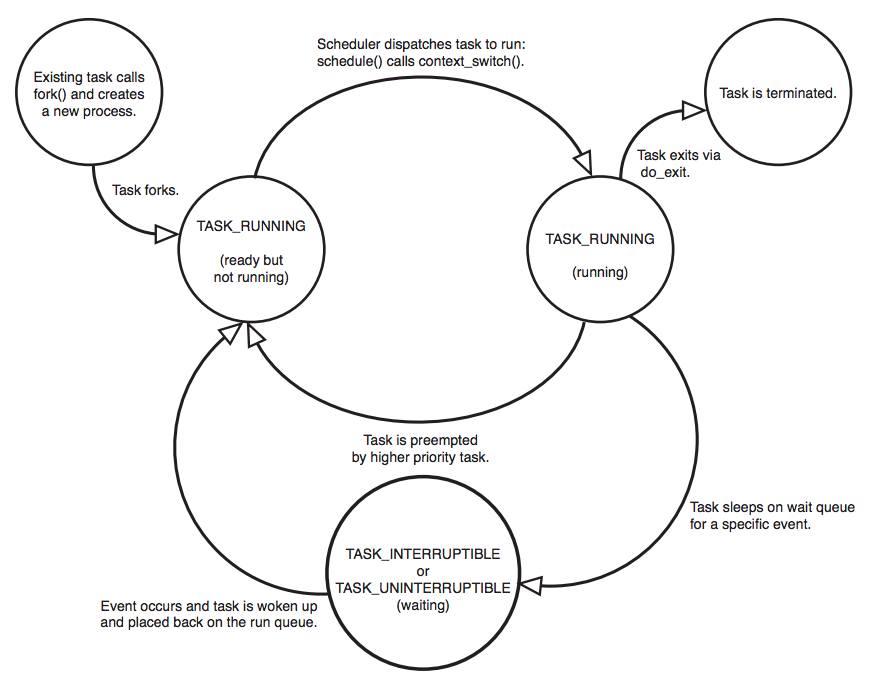
\includegraphics[width=\textwidth]{process_life} %add try_to_wake_up in the image or make a new one
\caption{State machine of task states}
\label{img:process_life}
\end{figure}

\chapter{The scheduler}
\label{ch:sched}

As we have seen before, the CPU can only execute one task at a time and even on multiprocessors systems, the number of task will be in most cases larger than the number of cores. For this reason we need a system to alternate the execution of the tasks, but how do we chose which task to run? This is the job of the scheduler, which we will now explore.

\section{Objectives of the scheduler}


% Citare altre schedulng class: SCHED_FIFO, SCHED_RR, SCHED_DEADLINE


The scheduler cannot simply choose the tasks in any order, there are some tasks that are highly time sensitive and needs to be executed as fast as possible, and tasks that can wait longer without any consequence The scheduler has to take this and many other aspects into consideration before making a decision.

%minimize response time and maximize throughput
\paragraph{Response time and throughput}
When the user interact with the system he expects it to react almost immediately, he doesn't want to wait a few seconds between the press of a button and the response from the system. So, one of the objectives of the scheduler is to \textbf{minimize the response time of the tasks}. 

%interactive tasks
Obviously we can have different types of tasks: a text editor, for example, will spend most of its time waiting for an input form the user, but when the user gives an input, we want the program to respond as fast as possible, we call this type of task \textit{interactive}.

%throughput
At the same time we want to do as few context switches as possible. Every time the scheduler performs one the CPU is not being used by any task. On the long run, if we perform frequent context switches, this will have an impact on the performance of the system. The \textbf{throughput} is the total amount of work completed in a unit of time, and we also want to maximize this value.

\paragraph{Fairness}
The scheduler should also try to achieve fairness, in the long run two task with the same priority should run for roughly the same amount of time. And it should be proportional to the runtime of tasks with other priorities. The scheduler should also be starvation free, meaning that every task should get at least some cpu time.

\paragraph{Different workloads}
Linux is used in all sort of machine, from desktop computer to high-end servers to mobile devices and the types of workloads can be very different. The scheduler should have good results in every scenario.

\label{sec:cfs}
\section{Why CFS?} 
%CFS philosophy
%What are the improvements?
% Probably just a bit of history about past schedulers such as O(1) and BFS
% Also actual reasons why CFS is good
% Problem when deciding which scheduler should be implemented: many people will be unhappy

\subsubsection{O(1) Scheduler}

CFS is the default scheduler of linux since the 2.6.23 release, as a replacement for the O(1) scheduler. To understand the advantages of CFS we first need to understand how the previous version works.

\paragraph{Priority} %What is the priority of a task
Each task has a priority which consists of a static and a dynamic priority. The static priority, which corresponds to the nice value, can have a value from -20 to 19, -20 being the highest priority and 19 the lowest. The dynamic priority ranges from -5 to +5, it is based on the interactiveness of the task: an interactive task (I/O bound) gets an higher priority than a non-interactive one (CPU bound). The scheduler uses an heuristic method to determine the interactiveness of a task, it is done by keeping track of the amount of time that a task spend sleeping.

\paragraph{Timeslice} %How are timeslices calulated
The O(1) scheduler is based on the concept of timeslice, this is the amount of time that a task runs on the CPU. Each priority level is mapped to a different timeslice, high priorities get mapped to bigger timeslices while low priorities get mapped to smaller timeslices. 
%TODO: add brief introduction to time

\paragraph{} %How O(1) works and downsides
The runnable tasks are stored in two priority queues, an active and an expired queue. At the beginning all the task are inside the active queue, the tasks run on the CPU, in order of priority, for the assigned timeslice, when a task finishes its timeslice it's moved into the expired queue. Once all the tasks have finished their timeslice, the two queues swap role and the process starts again.

(Needs to develop further)[In the O(1) scheduler the timeslices are calculated independently from the load of the system, if only two low priority tasks are present, they both get assigned a short timeslice. This results in more frequent context switches than necessary which slows down the system. To guarantee good interactiveness the O(1) scheduler uses complex heuristics to determine if a task is interactive or not. This results in more complex code and doesn't resolve the problem entirely.]

\subsubsection{Rotating Staircase DeadLine}

Con Kolivas proposed a new scheduler that that tries to solve the problems of the O(1) scheduler. The goal was to design a scalable scheduler that was completely fair to all processes and allowed the best possible interactivity.

The Rotating Staircase DeadLine scheduler or RSDL assigns a quota of runtime based on the priority of the task. The task at the highest priority level are then executed round-robin with each other, when a task finishes it's quota it is moved to the next priority level and it's given a new quota. The entire priority level also has an assigned quota, when that quota expires, all the process in this priority level are moved to the next one. When a task finishes all its quotas at each priority level, it is moved to the expired queue. When all the task have finished their quota, the expired queue becomes active and the process starts again.

RSDL doesn't measure the sleep time of the tasks in order to identify interactive tasks, those tasks spend most of the time sleeping so they consume a little portion of their quota. When they get woken up, they will probably be at a high priority level meaning that, in most cases, they only have to wait for the task in the current runqueue's priority level. This guarantees a low latency for interactive tasks. 

\subsubsection{CFS}
The CFS scheduler was developed by Ingo Molnár, he was inspired by the \textit{Rotating Staircase Deadline} scheduler developed by Con Kolivas. 

CFS does not use fixed timeslices and does not use any heuristic method to calculate the priority of a task. It tries to model an ideal multitasking CPU on real hardware. Ideally every task receives 1/n of the processor's time, where n is the number of runnable tasks. This results in simpler code that can handle nice values better than the previous scheduler, the preemption time is no longer fixed like in the O(1) scheduler, but it is variable.

In the following section we look in more detail how CFS works.

\section{How does CFS work?} 

As we already said, CFS tries to simulate an ideal multitasking CPU. Each process gets assigned a portion of the CPU depending on their weight, the weight is determined by the priority of the task (nice value).

\paragraph{Weight}
According to the documentation the weight is roughly equivalent to: $\dfrac{1024}{(1.25)^{nice}}$. This way an increase of 1 in the nice value roughly translates to a 10\% increase in CPU (with same load condition).%?

Write examples here, for 2 processes same nice and 2 processes with 1 nice difference

Plot the function here

%TODO: add explanation for this formula
Let's write the weight formula in a more readable format.
\begin{equation}
    w(n) = \frac{2^{10}}{(\frac{5}{4})^{n}}
\end{equation}

The percentage of CPU time given to a process is equal to its weight divided by the sum of all the other weights. Let's suppose we have only two processes and they have a difference in nice $d$, then the CPU percentage of the process with nice $n$ is:

\begin{equation}
    CPU_\% = \frac{w(n)}{w(n)+w(n+d)}
\end{equation}

Let's now plug in the weight formula and simplify. Where $\alpha=\frac{5}{4}$. 

\begin{align*}
    &\frac{w(n)}{w(n)+w(n+d)} =
    \frac{\dfrac{2^{10}}{\alpha^{n}}}{\dfrac{2^{10}}{\alpha^{n}}+\dfrac{2^{10}}{\alpha^{n+d}}} =\\
    &\frac{1}{\dfrac{2^{10}}{\alpha^{n}} \left(\dfrac{2^{10}}{\alpha^{n}}+\dfrac{2^{10}}{\alpha^{n+d}}\right)} =
    \frac{1}{1+\dfrac{\alpha^{n}}{\alpha^{n+d}}} =
    \frac{1}{1+\dfrac{1}{\alpha^{d}}}
\end{align*}

We have now a function to calculate the $CPU_\%$ of a process given a difference in nice. 

\begin{equation}
    CPU_\%(d)=\frac{1}{1+\left(\dfrac{4}{5}\right)^{d}}
\end{equation}

Let's plot this function.TODO

% \begin{tikzpicture}
%   \begin{axis}[] 
%     \addplot {1 / (1 + (4/5)^x)}; 
%   \end{axis}
% \end{tikzpicture}

Finally, we derive in 0 and we get $0.5log(5/4)$, which is roughly equivalent to 0.11157. This is the 10\% increase that was referred by the comments in the code.

\paragraph{Assigned time}
The actual time of CPU that the task gets is determined by the weight of the task, the total weight of all the tasks in the run queue, the \textit{target latency} and the \textit{minimum granularity}. 

\textit{Target latency} is the period of the scheduler and it's a tunable value, CFS tries to schedule every runnable task at least once in this period. 

\textit{Minimum granularity} is the minimum amount of time that can be assigned to a task, this is done to prevent small timeslices that would result in a higher switching cost.

The time assigned to a task is then equal to: $(target latency) * ((task's weight)/(total weight))$. %TODO: fix format

\paragraph{vruntime}

Tasks can be preempted at any time so, in order to know which task deserves to be run next, the scheduler needs to keep track of the amount of time that a task has spent running. This time is then weighted with the weight discussed before. This value is called the virtual runtime. The general formula for calculating the virtual runtime is: \\$delta\_exec * weight\_of\_nice\_0 / task\_weight$ %TODO: fix

If the nice value of the task is 0, then the virtual runtime is equivalent to the actual time spent running on the CPU.

If the nice value is less than 0, then the virtual runtime will be smaller the the actual runtime. This means that the vruntime of an high priority task will increase more slowly than the vruntime of a low priority one. So, in order to keep all the virtual runtimes at the same level the high priority task will have to run for more time.

On the other hand, if the nice value is more than 0, the virtual runtime will increase faster.

\paragraph{Running the next task}

As we said before, the goal of CFS is to be as fair as possible with all the task. This means keeping all the task's vruntime as close as possible to each other. Following this logic, the task that deserves more than anyone to be executed next, is the one with the smallest vruntime.

% Spostare in Implementation il Red-Black tree
\paragraph{Red-Black Tree}
%do we need an introduction on how red-black trees works?
The runnable tasks are stored inside a red-black tree, this allows us to perform efficienty many of the function that we need.
%basics of red-black trees
A Red-black Tree is a type of self-balancing binary search tree, this means that the insertion and the deletion of an element try to keep the height of the tree as small as possible. This characteristic is important because the cost of the most common functions (search, insertion and deletion) is proportional to the height of the tree, in this case log(n) where n is the number of nodes in the tree.
%how is it used in cfs
As we said before, the task to run next, is the one with the smallest vruntime, in a red-black tree this is the task corresponding to the leftmost node of tree. (In reality we don't traverse the tree, we cache the leftmost node in order to retrieve it faster).

\section{Time Management}%Introduction on time management
Many functions of the kernel need to keep track of the passing of the time. The scheduler, for example, needs to know for how long a task has been running in order to know when to preempt it and give the control of the CPU to another task. But there are many other functions that are time-driven, so it's important to understand how the system keeps track of the time.

The kernel requires an hardware timer to manage the passing of time. This timer can be implemented in different ways and there can be more timers in a system, but the general idea is the same: the timer sends an interrupt at a fixed frequency known by the kernel, this way it also knows the time between two timer interrupts and can perform periodic actions such as updating the system uptime. The period between two interrupt is called a \textit{tick} and the frequency is called \textit{tick rate}, this value inside the kernel is defined as \textbf{HZ}. If the value of HZ is 100, it means that the frequency is 100HZ and there is a tick every $1/100$ seconds, or 10 milliseconds.

\subsubsection{Choice of the tick rate}
As we will see later, many parts of the system are time-dependant, so they rely on the timer interrupt. Changing the frequency of the interrupt can have a large impact on the behavior of the system, there are pros and cons to larger an smaller values oh HZ.

%pros of larger HZ
A larger HZ means that the timer interrupt has a finer resolution, which means that all the timed events also have a higher resolution and also allows to improve the accuracy of those events. As an example, let's consider process preemption, with an higher tick rate we can improve the accuracy and reduce the scheduling latency. Suppose that a process has 2 milliseconds left of its timeslice and the timer interrupt has just occurred, with an HZ of 100 the next interrupt will occur in 10 milliseconds, giving the process 8 extra milliseconds, it also means that another task has to wait for more time in the runqueue and this can be an issue for time-sensitive tasks. With a larger HZ, 1000 for example, in the worst case scenario, the latency is only 1 millisecond.

%cons of larger HZ
There is also a drawback to increasing the tick rate: the interrupt handler gets executed more often and results in less processor time for the tasks. The actual impact of the increased overhead is debatable and depends on the speed of the processor.

%different values of HZ
The value of HZ depends on the hardware and on the configuration of the machine. On i386 HZ had a value of 100, with linux version 2.6 the value was raised to 1000 and later was made a configurable parameter and the default became 250. With the time were also introduced other, more accurate, timers, making an high HZ less necessary. It is also possible to configure the kernel as \textit{tickless} (NO\_HZ), this means that the interrupt is no longer at fixed intervals, but it's dynamically scheduled as needed, which is helpful for power savings.

\subsubsection{Jiffies}
%What is jiffies
\textit{Jiffies} is the number of ticks that have occurred since the system started, very time that the interrupt handler is executed, the value of \textit{jiffies} is increased by one. This means that if we know the value of HZ and the value of jiffies we can theoretically convert from seconds to jiffies, simply by doing \verb|seconds * HZ| and from jiffies to seconds with: jiffies / HZ
%TODO: code for conversion here
%add more about implementation

\paragraph{sched\_clock()}

An important function of the kernel is sched\_clock(), it returns the system's uptime in nanoseconds. An architecture may provide an implementation, but if it is not provided, the system will use the jiffies counter to calculate the system's uptime.

The scheduler uses this function to determine the absolute time that the current task has been running. If the system uses the jiffies counter to determine this value the maximum resolution of sched\_clock() depends on the value of HZ. In this case the choice of HZ becomes more relevant.

\subsubsection{Interrupt Handler}

As we said before, the interrupt handler gets called at fixed intervals (unless configured with NO\_HZ). The handler perform many important functions, some of this actions depend on the architecture of the system, but some are independent and are executed by the \textit{periodic\_tick()} function (in \textit{kernel/time/tick\_common.c}):

\begin{code}
static void tick_periodic(int cpu)
{
	if (tick_do_timer_cpu == cpu) {
		write_seqlock(&jiffies_lock);

		/* Keep track of the next tick event */
		tick_next_period = ktime_add(tick_next_period, tick_period);

		do_timer(1);
		write_sequnlock(&jiffies_lock);
		update_wall_time();
	}

	update_process_times(user_mode(get_irq_regs()));
	profile_tick(CPU_PROFILING);
}
\end{code}
The two most important functions here are do\_timer(1) and update\_process\_times. The first one increments the value of jiffies and updates the load statistics for the system.

The second is the most important for the scheduler, it updates various statistics and updates the runtime of the current task, if the task has finished its timeslice, it prompts a reschedule. We will see later in more detail how this works. % or should i put it here?
\begin{itemize} %to remove, just notes
\item updates\_process\_times (kernel/time/timer.c)
\item scheduler\_tick (kernel/sched/core.c)
\item sched\_clock\_tick (kernel/time/clock.c)
\item task\_tick (kernel/sched/fair.c)
\item entity\_tick 
\item update\_curr
\item check\_preempt\_tick
\end{itemize}

\section{Updating vruntime}



\chapter{Event tracing with ftrace} %Where do i put this section?
\label{chap:ftrace}


\chapter{Implementation}
\label{chap:implementation}
%Scheduling classes table (move this up)
\begin{tabular}{|c|c|}
\hline
\textbf{Scheduling classes} & \textbf{Scheduling policies}\\
\hline
stop\_sched\_class &\\
\hline
dl\_sched\_class   & SCHED\_DEADLINE\\
\hline
rt\_sched\_class   & SCHED\_FIFO \\
                   		   & SCHED\_RR\\
\hline
fair\_sched\_class & SCHED\_NORMAL\\
                   & SCHED\_BATCH\\
                   & SCHED\_IDLE\\
\hline
idle\_sched\_class &\\          
\hline
\end{tabular}


\section{Structs and their role}
\paragraph{The process descriptor}
\paragraph{thread\_info}
\paragraph{mm\_struct}
%kernel threads have mm at null
% task\_strt
%Need to explain mm_struct and some memory management
% explain kernel stacks -> thread\_info and current macro (only valid in process context in kernel)
%kernel preemption and user preemptio, returning to userspace (entry.S which defines entry and exit instruction)
\section{Core} 
\label{sec:core}
Explain address spaces, kernel threads and user threads, maybe mm\_struct
%arch/x86/entry/entry_64.S explain kernel preemption e user preemption
\section{Scheduler routines} 
%If there are events in the fuction, explain them (events directly related to scheduling)
\subsubsection{enqueue\_task()}

\subsubsection{schedule()}

\subsubsection{context\_switch()}

\section{Other events} %Not directly related to scheduling
\label{sec:other_events}
Tracepoints, file and line
\begin{verbatim}
fs/exec.c:1698:		trace_sched_process_exec(current, old_pid, bprm);

kernel/exit.c:1503:	trace_sched_process_wait(wo->wo_pid);
kernel/exit.c:180:	trace_sched_process_free(tsk);
kernel/exit.c:866:	trace_sched_process_exit(tsk);

kernel/fork.c:2242:	trace_sched_process_fork(current, p);

kernel/hung_task.c:113:	trace_sched_process_hang(t);

kernel/kthread.c:543:	trace_sched_kthread_stop(k);
kernel/kthread.c:554:	trace_sched_kthread_stop_ret(ret);
kernel/kthread.c:554:	trace_sched_kthread_stop_ret(ret);

kernel/sched/core.c:1171:	trace_sched_migrate_task(p, new_cpu);
kernel/sched/core.c:1295:	trace_sched_swap_numa(cur, arg.src_cpu, p, arg.dst_cpu);
kernel/sched/core.c:1358:		trace_sched_wait_task(p);
kernel/sched/core.c:1659:	trace_sched_wakeup(p);
kernel/sched/core.c:1798:			trace_sched_wake_idle_without_ipi(cpu);
kernel/sched/core.c:1813:		trace_sched_wake_idle_without_ipi(cpu);
kernel/sched/core.c:1970:	trace_sched_waking(p);
kernel/sched/core.c:2100:	trace_sched_waking(p);
kernel/sched/core.c:2425:	trace_sched_wakeup_new(p);
kernel/sched/core.c:2425:	trace_sched_wakeup_new(p);
kernel/sched/core.c:3469:		trace_sched_switch(preempt, prev, next);
kernel/sched/core.c:3797:	trace_sched_pi_setprio(p, pi_task);
kernel/sched/core.c:473:		trace_sched_wake_idle_without_ipi(cpu);
kernel/sched/core.c:545:		trace_sched_wake_idle_without_ipi(cpu);
kernel/sched/core.c:5485:	trace_sched_move_numa(p, curr_cpu, target_cpu);

kernel/sched/fair.c:1836:			trace_sched_stick_numa(p, env.src_cpu, env.best_cpu);
kernel/sched/fair.c:1844:		trace_sched_stick_numa(p, env.src_cpu, task_cpu(env.best_task));
kernel/sched/fair.c:3817:	if (trace_sched_stat_wait_enabled()    ||
kernel/sched/fair.c:3818:			trace_sched_stat_sleep_enabled()   ||
kernel/sched/fair.c:3819:			trace_sched_stat_iowait_enabled()  ||
kernel/sched/fair.c:3820:			trace_sched_stat_blocked_enabled() ||
kernel/sched/fair.c:3821:			trace_sched_stat_runtime_enabled())  {
kernel/sched/fair.c:833:		trace_sched_stat_runtime(curtask, delta_exec, curr->vruntime);
kernel/sched/fair.c:886:		trace_sched_stat_wait(p, delta);
kernel/sched/fair.c:925:			trace_sched_stat_sleep(tsk, delta);
kernel/sched/fair.c:944:				trace_sched_stat_iowait(tsk, delta);
kernel/sched/fair.c:947:			trace_sched_stat_blocked(tsk, delta);
\end{verbatim}
Events details + comments found in the code
\begin{verbatim}
/*
 * Tracepoint for calling kthread_stop, performed to end a kthread:
 */
sched_kthread_stop

/*
 * Tracepoint for the return value of the kthread stopping:
 */
sched_kthread_stop_ret

/*
 * Tracepoints for waking up a task:
 */

/*
 * Tracepoint called when waking a task; this tracepoint is guaranteed to be
 * called from the waking context.
 */
sched_waking:
  ./kernel/sched/core.c:1970:
    try_to_wake_up - wake up a thread
  ./kernel/sched/core.c:2100:
    try_to_wake_up_local - try to wake up a local task with rq lock held

/*
 * Tracepoint called when the task is actually woken; p->state == TASK_RUNNNG.
 * It it not always called from the waking context.
 */
sched_wakeup(./kernel/sched/core.c:1659):
  Mark the task runnable and perform wakeup-preemption.

/*
 * Tracepoint for waking up a new task:
 */
sched_wakeup_new(./kernel/sched/core.c:2425):
 wake_up_new_task - wake up a newly created task for the first time.
   This function will do some initial scheduler statistics housekeeping
   that must be done for every newly created context, then puts the task
   on the runqueue and wakes it.

/*
 * Tracepoint for task switches, performed by the scheduler:
 */
sched_switch(./kernel/sched/core.c:3469):
  context_switch - switch to the new MM and the new thread's register state.

/*
 * Tracepoint for a task being migrated:
 */
sched_migrate_task(./kernel/sched/core.c:1171):
  set_task_cpu(struct task_struct *p, unsigned int new_cpu)
  Migrate a task to new_cpu.

/*
 * Tracepoint for freeing a task:
 */
sched_process_free(./kernel/exit.c:180):
  TODO

/*
 * Tracepoint for a task exiting:
 */
sched_process_exit(./kernel/exit.c:866):
  process exit

/*
 * Tracepoint for waiting on task to unschedule:
 */
sched_wait_task

/*
 * Tracepoint for a waiting task:
 */
sched_process_wait(./kernel/exit.c:1503):

/*
 * Tracepoint for do_fork:
 */
sched_process_fork: (./kernel/fork.c:2242)
  _do_fork
    It copies the process, and if successful kick-starts                                                                                                   
    it and waits for it to finish using the VM if required.

/*
 * Tracepoint for exec:
 */
sched_process_exec(./fs/exec.c:1698):
  exec_binprm(struct linux_binprm *bprm)
  load binaries using bprm(binary parameter)

/*
 * Tracepoint for accounting wait time (time the task is runnable
 * but not actually running due to scheduler contention).
 */
sched_stat_wait

/*
 * Tracepoint for accounting sleep time (time the task is not runnable,
 * including iowait, see below).
 */
sched_stat_sleep

/*
 * Tracepoint for accounting iowait time (time the task is not runnable
 * due to waiting on IO to complete).
 */
sched_stat_iowait

/*
 * Tracepoint for accounting blocked time (time the task is in uninterruptible).
 */
sched_stat_blocked

/*
 * Tracepoint for accounting runtime (time the task is executing
 * on a CPU).
 */
sched_stat_runtime(./kernel/sched/fair.c:829):
  Update the current task's runtime statistics.

/*
 * Tracepoint for showing priority inheritance modifying a tasks
 * priority.
 */
sched_pi_setprio

/*
 * Detect Hung Task
 */
sched_process_hang(./kernel/hung_task.c:113):
  Kernel thread for detecting tasks stuck in D state

/*
 * Tracks migration of tasks from one runqueue to another. Can be used to
 * detect if automatic NUMA balancing is bouncing between nodes
 */
sched_move_numa

//TODO
sched_stick_numa

//TODO
sched_swap_numa

/*
 * Tracepoint for waking a polling cpu without an IPI.
 */
sched_wake_idle_without_ipi
\end{verbatim}
\begin{thebibliography}{}
\bibitem{ritchie}
AT\&T Bell Labs promotional film, circa 1980
\textit{Ken Thompson and Dennis Ritchie Explain UNIX (Bell Labs)} %well, this is a youtube video, should i even cite this?

\bibitem{cesati}
Marco Cesati and Daniel P. Bovet.
\textit{Understanding the Linux Kernel, Third Edition}.
O'reilly, 2005.

\bibitem{pid_h}
Comments in \verb|include/linux/kernel.h|
\end{thebibliography}
\end{document}

\section{Testing}
%just testing equations etc
\begin{equation}
    nice\in[-19 \dots 20]
\end{equation}
\begin{equation}
    timeslice\in[granularity_{min} \dots period]
\end{equation}
\begin{equation}
    weight=\frac{1024}{1.25^{nice}}
\end{equation}
\begin{equation}
    timeslice(task)=period\frac{weight(task)}{weight(rq)}
\end{equation}
\begin{equation}
    CPU_\%(task)=\frac{weight(task)}{weight(rq)}
\end{equation}
\begin{equation} \label{eq_gran}
    granularity=\frac{latency}{n_{running}} - \frac{latency}{\cfrac{n_{running}}{n_{running}}}
\end{equation}
The equation \ref{eq_gran} expresses the relation between latency and granularity.

In the code these values are called respectively \verb|sysctl_sched_latency| and \verb|sysctl_sched_min_granularity|.
\begin{code}
static u64 __sched_period(unsigned long nr_running){
if(unlikely(nr_running > sched_nr_latency))
	return nr_running * sysctl_sched_min_granularity;
else
	return sysctl_sched_latency;
}
\end{code}
This is how the scheduling period is calculated.\\ 
\verb|sched_nr_latency| is simply $\cfrac{latency}{granularity_{min}}$.
\begin{code}
#define likely(x)       __builtin_expect(!!(x), 1)
#define unlikely(x)     __builtin_expect(!!(x), 0)
\end{code}
Branch prediction macros definition (\verb|include/linux/compiler.h|), the double inversion is to make sure the parameter is binary

\begin{equation}
    lantency = 6ms(1 + \log_2 n_{CPU})
\end{equation}
Default latency.
\begin{equation}
    granularity = 0.75ms(1 + \log_2 n_{CPU})
\end{equation}
Default granularity.

%FUNCTIONS CODE

\begin{code}
void scheduler_tick(void) //If current task needs to be scheduled out, then TIF_NEED_RESCHED flag is set for it
{
	int cpu = smp_processor_id();
	struct rq *rq = cpu_rq(cpu);
	struct task_struct *curr = rq->curr;
	struct rq_flags rf;

	sched_clock_tick();

	rq_lock(rq, &rf);

	update_rq_clock(rq);
	curr->sched_class->task_tick(rq, curr, 0);
	cpu_load_update_active(rq);
	calc_global_load_tick(rq);
	psi_task_tick(rq);

	rq_unlock(rq, &rf);

	perf_event_task_tick();

#ifdef CONFIG_SMP
	rq->idle_balance = idle_cpu(cpu);
	trigger_load_balance(rq);
#endif
}
\end{code}
\begin{code}
static void task_tick_fair(struct rq *rq, struct task_struct *curr, int queued){
	struct cfs_rq *cfs_rq;
	struct sched_entity *se = &curr->se;

	for_each_sched_entity(se) {
		cfs_rq = cfs_rq_of(se);
		entity_tick(cfs_rq, se, queued);
	}

	if (static_branch_unlikely(&sched_numa_balancing))
		task_tick_numa(rq, curr);

	update_misfit_status(curr, rq);
}
\end{code}
\begin{code}
static void entity_tick(struct cfs_rq *cfs_rq, struct sched_entity *curr, int queued){
	update_curr(cfs_rq);
	update_load_avg(cfs_rq, curr, UPDATE_TG);
	update_cfs_group(curr);
	// ... roba hrtimer
	if (cfs_rq->nr_running > 1)
		check_preempt_tick(cfs_rq, curr);	
}	
\end{code}
\begin{code}
//First, it determines time slice for the current task
//Second, it set resched flag on current task if either of two conditions are satisifed
//(a) if current task has run beyond its time slice
//(b) if current task vruntime exceeds next task vruntime by time slice, provided time run by current task is more than sysctl_sched_min_granularity
static void check_preempt_tick(struct cfs_rq *cfs_rq, struct sched_entity *curr){
	unsigned long ideal_runtime, delta_exec;
	struct sched_entity *se;
	s64 delta;

	ideal_runtime = sched_slice(cfs_rq, curr);
	delta_exec = curr->sum_exec_runtime - curr->prev_sum_exec_runtime;//Why doesn't this use calc_delta_fair()?
	if (delta_exec > ideal_runtime) {
		resched_curr(rq_of(cfs_rq));
		/*
		 * The current task ran long enough, ensure it doesn't get
		 * re-elected due to buddy favours.
		 */
		clear_buddies(cfs_rq, curr);
		return;
	}

	/*
	 * Ensure that a task that missed wakeup preemption by a
	 * narrow margin doesn't have to wait for a full slice.
	 * This also mitigates buddy induced latencies under load.
	 */
	if (delta_exec < sysctl_sched_min_granularity)
		return;

	se = __pick_first_entity(cfs_rq);
	delta = curr->vruntime - se->vruntime;

	if (delta < 0) //Curr vruntime is less than the next task's vruntime
		return;

	if (delta > ideal_runtime) //Current task vruntime exceeded next task vruntime by a full time slice
		resched_curr(rq_of(cfs_rq));
}
\end{code}
\begin{code}
static u64 sched_slice(struct cfs_rq *cfs_rq, struct sched_entity *se){
	u64 slice = __sched_period(cfs_rq->nr_running + !se->on_rq);

	for_each_sched_entity(se) {
		struct load_weight *load;
		struct load_weight lw;

		cfs_rq = cfs_rq_of(se);
		load = &cfs_rq->load;

		if (unlikely(!se->on_rq)) {
			lw = cfs_rq->load;

			update_load_add(&lw, se->load.weight);
			load = &lw;
		}
		slice = __calc_delta(slice, se->load.weight, load);
	}
	return slice;
}
\end{code}
\begin{code}
static u64 __sched_period(unsigned long nr_running){
	if (unlikely(nr_running > sched_nr_latency))
		return nr_running * sysctl_sched_min_granularity;
	else
		return sysctl_sched_latency;
}
\end{code}
\begin{code}
static void update_curr(struct cfs_rq *cfs_rq) //This is __update_curr{
	//Updates vruntime of curr using calc_delta_fair
	struct sched_entity *curr = cfs_rq->curr;
	u64 now = rq_clock_task(rq_of(cfs_rq));
	u64 delta_exec;

	if (unlikely(!curr))
		return;

	delta_exec = now - curr->exec_start; //time elapsed since the last time we called update_curr
	if (unlikely((s64)delta_exec <= 0))
		return;

	curr->exec_start = now;

	schedstat_set(curr->statistics.exec_max,
		      max(delta_exec, curr->statistics.exec_max));

	curr->sum_exec_runtime += delta_exec; //actual runtime
	schedstat_add(cfs_rq->exec_clock, delta_exec);

	curr->vruntime += calc_delta_fair(delta_exec, curr); //fairly scaled runtime
	update_min_vruntime(cfs_rq);

	if (entity_is_task(curr)) {
		struct task_struct *curtask = task_of(curr); //uses container_of

		trace_sched_stat_runtime(curtask, delta_exec, curr->vruntime);
		cgroup_account_cputime(curtask, delta_exec);
		account_group_exec_runtime(curtask, delta_exec);
	}

	account_cfs_rq_runtime(cfs_rq, delta_exec); //adds to the total runtime
}
\end{code}
\begin{code}
/*
 * delta /= w
 */
static inline u64 calc_delta_fair(u64 delta, struct sched_entity *se){
	if (unlikely(se->load.weight != NICE_0_LOAD))
		delta = __calc_delta(delta, NICE_0_LOAD, &se->load); //Scale it fairly, basically delta = delta_exec * NICE_0_LOAD / curr->load.weight;

	return delta; //Do not scale delta with the weighting factor
}
\end{code}
\begin{code}
asmlinkage __visible void __sched schedule(void){
	struct task_struct *tsk = current;

	sched_submit_work(tsk);
	do {
		preempt_disable();
		__schedule(false);
		sched_preempt_enable_no_resched();
	} while (need_resched());
}
\end{code}
\begin{code}
//min_vruntime = MAX(min_vruntime, MIN(current_running_task.vruntime, cfs_rq.left_most_task.vruntime))
//So: the max is there to ensure that min_vruntime is increasing monothonically, it should never go backwards!
static void update_min_vruntime(struct cfs_rq *cfs_rq){
	struct sched_entity *curr = cfs_rq->curr;
	struct rb_node *leftmost = rb_first_cached(&cfs_rq->tasks_timeline);

	u64 vruntime = cfs_rq->min_vruntime;

	if (curr) {
		if (curr->on_rq)
			vruntime = curr->vruntime;
		else
			curr = NULL;
	}

	if (leftmost) { /* non-empty tree */
		struct sched_entity *se;
		se = rb_entry(leftmost, struct sched_entity, run_node);

		if (!curr)
			vruntime = se->vruntime;
		else
			vruntime = min_vruntime(vruntime, se->vruntime);
	}

	/* ensure we never gain time by being placed backwards. */
	cfs_rq->min_vruntime = max_vruntime(cfs_rq->min_vruntime, vruntime);
}
\end{code}
\begin{code}
struct sched_entity *__pick_first_entity(struct cfs_rq *cfs_rq){
	struct rb_node *left = rb_first_cached(&cfs_rq->tasks_timeline);

	if (!left)
		return NULL;

	return rb_entry(left, struct sched_entity, run_node);
}
\end{code}

STRUCTS CODE
\begin{code}
#define MAX_NICE	19
#define MIN_NICE	-20
#define NICE_WIDTH	(MAX_NICE - MIN_NICE + 1)

#define MAX_USER_RT_PRIO	100
#define MAX_RT_PRIO		MAX_USER_RT_PRIO

#define MAX_PRIO		(MAX_RT_PRIO + NICE_WIDTH)
#define DEFAULT_PRIO		(MAX_RT_PRIO + NICE_WIDTH / 2)

/*
 * Convert user-nice values [ -20 ... 0 ... 19 ]
 * to static priority [ MAX_RT_PRIO..MAX_PRIO-1 ],
 * and back.
 */
#define NICE_TO_PRIO(nice)	((nice) + DEFAULT_PRIO)
#define PRIO_TO_NICE(prio)	((prio) - DEFAULT_PRIO)

/*
 * 'User priority' is the nice value converted to something we
 * can work with better when scaling various scheduler parameters,
 * it's a [ 0 ... 39 ] range.
 */
#define USER_PRIO(p)		((p)-MAX_RT_PRIO)
#define TASK_USER_PRIO(p)	USER_PRIO((p)->static_prio)
#define MAX_USER_PRIO		(USER_PRIO(MAX_PRIO))
\end{code}
\begin{code}
static void set_load_weight(struct task_struct *p, bool update_load){
	int prio = p->static_prio - MAX_RT_PRIO;
	struct load_weight *load = &p->se.load;

	/*
	 * SCHED_IDLE tasks get minimal weight:
	 */
	if (idle_policy(p->policy)) {
		load->weight = scale_load(WEIGHT_IDLEPRIO);
		load->inv_weight = WMULT_IDLEPRIO;
		p->se.runnable_weight = load->weight;
		return;
	}

	/*
	 * SCHED_OTHER tasks have to update their load when changing their
	 * weight
	 */
	if (update_load && p->sched_class == &fair_sched_class) {
		reweight_task(p, prio);
	} else {
		load->weight = scale_load(sched_prio_to_weight[prio]);
		load->inv_weight = sched_prio_to_wmult[prio];
		p->se.runnable_weight = load->weight;
	}
}
\end{code}
\begin{code}
//arch/x86/include/asm/thread_info.h
struct thread_info {
	unsigned long		flags;		/* low level flags */
	u32			status;		/* thread synchronous flags */
};
\end{code}
\begin{code}
static const int prio_to_weight[40] = {
/* -20 */ 88761, 71755, 56483, 46273, 36291,
/* -15 */ 29154, 23254, 18705, 14949, 11916,
/* -10 */ 9548, 7620, 6100, 4904, 3906,
/* -5 */ 3121, 2501, 1991, 1586, 1277,
/* 0 */ 1024, 820, 655, 526, 423,
/* 5 */ 335, 272, 215, 172, 137,
/* 10 */ 110, 87, 70, 56, 45,
/* 15 */ 36, 29, 23, 18, 15,
};
\end{code}
\begin{code}
//include/linux/thread_info.h
#ifdef CONFIG_THREAD_INFO_IN_TASK
/*
 * For CONFIG_THREAD_INFO_IN_TASK kernels we need <asm/current.h> for the
 * definition of current, but for !CONFIG_THREAD_INFO_IN_TASK kernels,
 * including <asm/current.h> can cause a circular dependency on some platforms.
 */
#include <asm/current.h>
#define current_thread_info() ((struct thread_info *)current)
#endif

// ...

/*
 * flag set/clear/test wrappers
 * - pass TIF_xxxx constants to these functions
 */

//set_tsk_need_resched(struct task_struct *tsk) in sched.h leads to this:
static inline void set_ti_thread_flag(struct thread_info *ti, int flag){
	set_bit(flag, (unsigned long *)&ti->flags);
}

//arch/x86/include/asm/current.h
#include <linux/compiler.h>
#include <asm/percpu.h>

#ifndef __ASSEMBLY__
struct task_struct;

DECLARE_PER_CPU(struct task_struct *, current_task);

static __always_inline struct task_struct *get_current(void)
{
	return this_cpu_read_stable(current_task);
}

#define current get_current()

//arch/x86/include/asm/percpu.h
/*
 * this_cpu_read() makes gcc load the percpu variable every time it is
 * accessed while this_cpu_read_stable() allows the value to be cached.
 * this_cpu_read_stable() is more efficient and can be used if its value
 * is guaranteed to be valid across cpus.  The current users include
 * get_current() and get_thread_info() both of which are actually
 * per-thread variables implemented as per-cpu variables and thus
 * stable for the duration of the respective task.
 */
#define this_cpu_read_stable(var)	percpu_stable_op("mov", var)

#define percpu_stable_op(op, var)			\
({							\
	typeof(var) pfo_ret__;				\
	switch (sizeof(var)) {				\
	case 1:						\
		asm(op "b "__percpu_arg(P1)",%0"	\
		    : "=q" (pfo_ret__)			\
		    : "p" (&(var)));			\
		break;					\
	case 2:						\
		asm(op "w "__percpu_arg(P1)",%0"	\
		    : "=r" (pfo_ret__)			\
		    : "p" (&(var)));			\
		break;					\
	case 4:						\
		asm(op "l "__percpu_arg(P1)",%0"	\
		    : "=r" (pfo_ret__)			\
		    : "p" (&(var)));			\
		break;					\
	case 8:						\
		asm(op "q "__percpu_arg(P1)",%0"	\
		    : "=r" (pfo_ret__)			\
		    : "p" (&(var)));			\
		break;					\
	default: __bad_percpu_size();			\
	}						\
	pfo_ret__;					\
})
\end{code}
\begin{code}
//include/sched.h
union thread_union {
#ifndef CONFIG_ARCH_TASK_STRUCT_ON_STACK
	struct task_struct task;
#endif
#ifndef CONFIG_THREAD_INFO_IN_TASK
	struct thread_info thread_info;
#endif
	unsigned long stack[THREAD_SIZE/sizeof(long)];
};
\end{code}
\begin{code}
struct task_struct {
#ifdef CONFIG_THREAD_INFO_IN_TASK
	/*
	 * For reasons of header soup (see current_thread_info()), this
	 * must be the first element of task_struct.
	 */
	struct thread_info		thread_info;
#endif
	/* -1 unrunnable, 0 runnable, >0 stopped: */
	volatile long			state;

	void				*stack;
	atomic_t			usage;
	/* Per task flags (PF_*), defined further below: */
	unsigned int			flags;
	unsigned int			ptrace;

    / ...
    
	/* Current CPU: */
	unsigned int			cpu;
#endif
	unsigned int			wakee_flips;
	unsigned long			wakee_flip_decay_ts;
	struct task_struct		*last_wakee;

	/*
	 * recent_used_cpu is initially set as the last CPU used by a task
	 * that wakes affine another task. Waker/wakee relationships can
	 * push tasks around a CPU where each wakeup moves to the next one.
	 * Tracking a recently used CPU allows a quick search for a recently
	 * used CPU that may be idle.
	 */
	int				recent_used_cpu;
	int				wake_cpu;
#endif
	int				on_rq;

	int				prio;
	int				static_prio;
	int				normal_prio;
	unsigned int			rt_priority;

	const struct sched_class	*sched_class; //Contains the task_tick function and other functions
											  //This contains a circular list of all scheduling classes
	struct sched_entity		se;
	struct sched_rt_entity		rt;
	
	// ...
	
	struct mm_struct		*mm;
	struct mm_struct		*active_mm;
	
	// ...
	
	/*
	 * Children/sibling form the list of natural children:
	 */
	struct list_head		children;
	struct list_head		sibling;
	struct task_struct		*group_leader;

	/*
	 * 'ptraced' is the list of tasks this task is using ptrace() on.
	 *
	 * This includes both natural children and PTRACE_ATTACH targets.
	 * 'ptrace_entry' is this task's link on the p->parent->ptraced list.
	 */
	struct list_head		ptraced;
	struct list_head		ptrace_entry;

	/* PID/PID hash table linkage. */
	struct pid			*thread_pid;
	struct hlist_node		pid_links[PIDTYPE_MAX];
	struct list_head		thread_group;
	struct list_head		thread_node;
	
	// ...
	
	char				comm[TASK_COMM_LEN];
};
\end{code}
\begin{code}
struct sched_entity { //Sched normal
	/* For load-balancing: */
	struct load_weight		load;
	unsigned long			runnable_weight;
	struct rb_node			run_node; //Node of this sched_entity
	struct list_head		group_node;
	unsigned int			on_rq;

	u64				exec_start; 	  //Last time update_curr() was executed, expressed in ns
	u64				sum_exec_runtime; //Actual runtime
	u64				vruntime;		  //Fairly scaled runtime
	u64				prev_sum_exec_runtime; //When a process is taken from the CPU, its current sum_exec_runtime value is preserved in prev_exec_runtime

	u64				nr_migrations;

	struct sched_statistics		statistics;

#ifdef CONFIG_FAIR_GROUP_SCHED
	int				depth;
	struct sched_entity		*parent;
	/* rq on which this entity is (to be) queued: */
	struct cfs_rq			*cfs_rq;
	/* rq "owned" by this entity/group: */
	struct cfs_rq			*my_q; //If this is a group then this will be its sub-runqueue
#endif

#ifdef CONFIG_SMP
	/*
	 * Per entity load average tracking.
	 *
	 * Put into separate cache line so it does not
	 * collide with read-mostly values above.
	 */
	struct sched_avg		avg; //Load average
#endif
};

#ifdef CONFIG_FAIR_GROUP_SCHED
/* An entity is a task if it doesn't "own" a runqueue */
#define entity_is_task(se)	(!se->my_q)
#else
#define entity_is_task(se)	1
#endif
\end{code}
\begin{code}
struct load_weight {
	unsigned long			weight;
	u32				inv_weight;
};
\end{code}
\begin{code}
/*
 * Helpers for converting nanosecond timing to jiffy resolution
 */
#define NS_TO_JIFFIES(TIME)	((unsigned long)(TIME) / (NSEC_PER_SEC / HZ))
\end{code}
\begin{code}
struct cfs_bandwidth {
#ifdef CONFIG_CFS_BANDWIDTH
	raw_spinlock_t		lock;
	ktime_t			period;
	u64			quota;
	u64			runtime;
	s64			hierarchical_quota;
	u64			runtime_expires;
	int			expires_seq;

	short			idle;
	short			period_active;
	struct hrtimer		period_timer;
	struct hrtimer		slack_timer;
	struct list_head	throttled_cfs_rq;

	/* Statistics: */
	int			nr_periods;
	int			nr_throttled;
	u64			throttled_time;

	bool                    distribute_running;
#endif
};
\end{code}
\begin{code}
struct sched_avg {
	u64				last_update_time;
	u64				load_sum;
	u64				runnable_load_sum;
	u32				util_sum;
	u32				period_contrib;
	unsigned long			load_avg;
	unsigned long			runnable_load_avg;
	unsigned long			util_avg;
	struct util_est			util_est;
} ____cacheline_aligned;
\end{code}
\begin{code}

\end{code}
\begin{code}
struct rq {
	/* runqueue lock: */
	raw_spinlock_t		lock;

	/*
	 * nr_running and cpu_load should be in the same cacheline because
	 * remote CPUs use both these fields when doing load calculation.
	 */
	unsigned int		nr_running;
#ifdef CONFIG_NUMA_BALANCING
	unsigned int		nr_numa_running;
	unsigned int		nr_preferred_running;
	unsigned int		numa_migrate_on;
#endif
	#define CPU_LOAD_IDX_MAX 5
	unsigned long		cpu_load[CPU_LOAD_IDX_MAX];
#ifdef CONFIG_NO_HZ_COMMON
#ifdef CONFIG_SMP
	unsigned long		last_load_update_tick;
	unsigned long		last_blocked_load_update_tick;
	unsigned int		has_blocked_load;
#endif /* CONFIG_SMP */
	unsigned int		nohz_tick_stopped;
	atomic_t nohz_flags;
#endif /* CONFIG_NO_HZ_COMMON */

	/* capture load from *all* tasks on this CPU: */
	struct load_weight	load;
	unsigned long		nr_load_updates;
	u64			nr_switches;

	struct cfs_rq		cfs;
	struct rt_rq		rt;
	struct dl_rq		dl;
    
    struct hrtimer		hrtick_timer; //High resolution timer
    // ...	
};
\end{code}
\begin{code}
struct cfs_rq {
	struct load_weight	load;
	unsigned long		runnable_weight;
	unsigned int		nr_running;
	unsigned int		h_nr_running;

	u64			exec_clock;
	u64			min_vruntime;
#ifndef CONFIG_64BIT
	u64			min_vruntime_copy;
#endif

	struct rb_root_cached	tasks_timeline; //rb_root
	//There is no struct rb_node *rb_leftmost; !!
	//Explaination: it gets calculated in update_min_vruntime() by rb_first_cached() (which is just a macro for (root)->rb_leftmost)

	/*
	 * 'curr' points to currently running entity on this cfs_rq.
	 * It is set to NULL otherwise (i.e when none are currently running).
	 */
	struct sched_entity	*curr;
	struct sched_entity	*next;
	struct sched_entity	*last;
	struct sched_entity	*skip;

#ifdef CONFIG_SMP
	/*
	 * CFS load tracking
	 */
	struct sched_avg	avg; //Load average
#ifndef CONFIG_64BIT
	u64			load_last_update_time_copy;
#endif
	struct {
		raw_spinlock_t	lock ____cacheline_aligned;
		int		nr;
		unsigned long	load_avg;
		unsigned long	util_avg;
		unsigned long	runnable_sum;
	} removed;

#ifdef CONFIG_FAIR_GROUP_SCHED
	unsigned long		tg_load_avg_contrib;
	long			propagate;
	long			prop_runnable_sum;

	/*
	 *   h_load = weight * f(tg)
	 *
	 * Where f(tg) is the recursive weight fraction assigned to
	 * this group.
	 */
	unsigned long		h_load;
	u64			last_h_load_update;
	struct sched_entity	*h_load_next;
#endif /* CONFIG_FAIR_GROUP_SCHED */
#endif /* CONFIG_SMP */

#ifdef CONFIG_FAIR_GROUP_SCHED
	struct rq		*rq;	/* CPU runqueue to which this cfs_rq is attached */

	/*
	 * leaf cfs_rqs are those that hold tasks (lowest schedulable entity in
	 * a hierarchy). Non-leaf lrqs hold other higher schedulable entities
	 * (like users, containers etc.)
	 *
	 * leaf_cfs_rq_list ties together list of leaf cfs_rq's in a CPU.
	 * This list is used during load balance.
	 */
	int			on_list;
	struct list_head	leaf_cfs_rq_list;
	struct task_group	*tg;	/* group that "owns" this runqueue */

#ifdef CONFIG_CFS_BANDWIDTH
	int			runtime_enabled;
	int			expires_seq;
	u64			runtime_expires;
	s64			runtime_remaining;

	u64			throttled_clock;
	u64			throttled_clock_task;
	u64			throttled_clock_task_time;
	int			throttled;
	int			throttle_count;
	struct list_head	throttled_list;
#endif /* CONFIG_CFS_BANDWIDTH */
#endif /* CONFIG_FAIR_GROUP_SCHED */
};
\end{code}
\begin{code}
struct sched_class {
	const struct sched_class *next;

	void (*enqueue_task) (struct rq *rq, struct task_struct *p, int flags);
	void (*dequeue_task) (struct rq *rq, struct task_struct *p, int flags);
	void (*yield_task)   (struct rq *rq);
	bool (*yield_to_task)(struct rq *rq, struct task_struct *p, bool preempt);

	void (*check_preempt_curr)(struct rq *rq, struct task_struct *p, int flags);

	/*
	 * It is the responsibility of the pick_next_task() method that will
	 * return the next task to call put_prev_task() on the @prev task or
	 * something equivalent.
	 *
	 * May return RETRY_TASK when it finds a higher prio class has runnable
	 * tasks.
	 */
	struct task_struct * (*pick_next_task)(struct rq *rq,
					       struct task_struct *prev,
					       struct rq_flags *rf);
	void (*put_prev_task)(struct rq *rq, struct task_struct *p);

#ifdef CONFIG_SMP
	int  (*select_task_rq)(struct task_struct *p, int task_cpu, int sd_flag, int flags);
	void (*migrate_task_rq)(struct task_struct *p, int new_cpu);

	void (*task_woken)(struct rq *this_rq, struct task_struct *task);

	void (*set_cpus_allowed)(struct task_struct *p,
				 const struct cpumask *newmask);

	void (*rq_online)(struct rq *rq);
	void (*rq_offline)(struct rq *rq);
#endif

	void (*set_curr_task)(struct rq *rq);
	void (*task_tick)(struct rq *rq, struct task_struct *p, int queued);
	void (*task_fork)(struct task_struct *p);
	void (*task_dead)(struct task_struct *p);
};
\end{code}

%DELETED PARTS:
%%%%%%%%%%%%%%%%
%where do i put this?
%move the following section elsewhere, maybe after explaining context switch, so that you can explain why there's no actual CS when calling a syscall
To get an idea of what a system call is doing at a lower level, let's look at this code which shows an example of both approaches. 
\begin{code}
#include <stdio.h>
#include <fcntl.h>
/* Direct system call */
int fd = syscall(SYS_open, "example.txt", O_WRONLY);
syscall(SYS_close, fd);
/* Calling glibc wrapper function */
fd = open("example.txt", O_WRONLY);
close(fd);
\end{code}
To be precise, the most direct way to invoke the system call would be to manually fill the registers yourself using assembly, which is obviously not portable. \verb|syscall()| essentially does this, the first argument of \verb|syscall()| is just the system call identifier, what it does is: 
\begin{enumerate}
\item Save the current CPU registers
\item Switches privilege mode as described before, but maintaining user context, no context switch happens
\item Depending on your architecture, fills the correct CPU registers with the syscall id and its arguments, then performs the syscall
\item Restores the saved CPU registers
\end{enumerate}

%%%%%%%%%%%%%%%%%%%%%%%%
\subsection{Source files organization} %Maybe move this section https://notes.shichao.io/lkd/ch2/#the-kernel-source-tree
Most header files included throughout the kernel code are located in the \verb|include/linux| directory. The architecture independent core logic of the kernel can be found in \verb|kernel|. Some of the source files located here have a 1-1 correspondence with the headers files in \verb|./include/linux|, in general all these headers will get included within these source files.\\
Some of the most important folders found in the root directory are:
\begin{itemize}
\item \textit{arch}

Architecture dependent code, with a subdirectory for each supported architecture. Most of the assembly code can be found here, there are no assembly files because all of the assembly code is inserted inline in C source files. This is a feature of \verb|gcc| which allows to insert arbitrary assembly in the code by using the builtin function \verb|__asm__()|. %how much percent?
\item \textit{drivers}

Device drivers, most of the kernel code is located here. Because of this, Linux can run on most systems without the need of additional, manually installed drivers (except for proprietary drivers, depending on the distribution). As of today this folder alone represents 60\% of the source code.
\item \textit{fs}

Filesystem and Virtual File System implementation. Block devices code is located in \textit{block}.
\item \textit{include}

Header files.
\item \textit{init}

TODO init routine executed in userspace...
\item \textit{ipc}

All of the interprocess communication mechanisms are implemented here.
\item \textit{kernel}

Most of the kernel core logic and architecture independent code. Some of the subdirectories correspond to whole subsystems or parts of core kernel mechanisms, Some examples are: 
\begin{itemize}
    \item \textit{sched} - Scheduling
    \item \textit{irq} - Interrupts
    \item \textit{trace} - Function and event tracing
    \item \textit{locking} - Synchronization
    \item \textit{time} - Jiffies and HRT (high resolution times)
\end{itemize}
There are also source files in the main directory that implement important functions such as \verb|fork.c|, \verb|exit.c|, \verb|pid.c|, \verb|panic.c| and \verb|sysctl.c|.
\item \textit{mm}

Memory management code. It contains the logic behind pagination, memory mapping, virtual memory and memory allocation. It's here that the SLUB allocator code lives, its job is to allocate memory for kernel threads while minimizing fragmentation. %check this
\item \textit{net}

All the protocols used for networking and the network stack are implemented here.
\end{itemize}
The code that we will see is located mostly in the \verb|include|,  \verb|kernel|, and \verb|kernel/sched| directories. This is architecture independent code and its headers, as expected from the code that implements process scheduling. As we will see later there is actually a very small piece of architecture dependent code: the function to get the address of the currently running process on a CPU.

%%%%%%%%%%%%%%%%%%%%
A process terminates by executing \verb|exit()| or when it receives SIGKILL or SIGTERM signals from another process, upon exit its \verb|task_struct| gets immediately deallocated. After the deallocation, the process will have an \textit{exit state}, this will initially be the \textit{zombie} state. A zombie process is a process that terminated, so it has no resources allocated, but its entry in the pid hash table is still present. It will be easily accessible through a table lookup, this is why zombie tasks are visible when showing processes with \verb|ps -aux|, even though they have exited. Tasks are not removed immediately from the hash table because the father process may want to access some of their information, such as their exit status, which is still present in memory. This actually very small resource leak because only the \verb|struct pid| (referred by the hash table) is still allocated, but it's a very small structure, occupying just a couple of bytes. If the hash table were to reference entire process descriptors, then \verb|exit()| could not deallocate the \verb|task_struct| and a big chunk of memory would stay allocated for a zombie process until it is reaped. Precisely, a \verb|task_struct| plus its kernel stack consumes around 10K of low kernel memory, that is \verb|THREAD_SIZE + sizeof(struct task_struct)|, assuming that kernel stacks are 8K in size, more on this in section \ref{chap:core}.